
While models such as the Building Game treat assembly intermediates as idealized structures, the intermediates of the physical application we are trying to model may face a chaotic and volatile range of forces. To more realistically model the ways in which our intermediate might flex and move under these forces, we impose a constraint model in with the rigidity of individual components of an intermediate are assumed, but in which the edges at which they meet are treated like a hinge. This constraint system specifies the ways in which an intermediate has freedom to move if it is able to move at all. A physically motivated way of addressing questions that the discrete models themselves are not adequate to answer is provided by this framework.   

\subsection{Configuration Space}

To characterize the freedoms of three-dimensional intermediates composed of rigid two-dimensional faces and connected at hinged edges, we parameterize each face and impose constraints in parameter space. Theoretically, the location and orientation of each face of an intermediate can be parameterized by six parameters: three for translation, three for rotation. This means the configuration of the entire intermediate can be represented by at most $6|F|$ parameters. In practice, however, it is often advantageous for ease of analysis and computational implementation to use more parameters to represent a given configuration. Often times, we use $3$ parameters to represent the location each vertex of each face, even if some of these vertices share common locations. This means that we often have an ambient parameter space of $\mathbb{R}^N$ with $N > 6|F|$. 

Upon this parameter space we place three types of constraints. The first removes the configuration's 6 trivial degrees of freedom due to translation and rotation. Since the intermediate is connected, this can be achieved by fixing the parameters of one of the intermediate's faces. Additionally, we enforce a rigidity constraint on each face ensuring that the structure of a constituent face will not change with movement of the larger structure. The final type of constraint ensures that the connections between two faces have hinge-like mobility. Since a shared edge has two vertices belonging to each face, this constraint is imposed by identifying the corresponding vertex locations. 

The \textit{configuration space} is defined to be the subset of ambient space $\left\{z \in \mathbb{R}^N : \varphi\left(z\right) = 0\right\}$  for which all $M$ of the constraint equations $\varphi: \mathbb{R}^N \to  \mathbb{R}^M $ are satisfied.  Since it is assumed that the standard configuration of the intermediate given by the model satisfies the constraints, the configuration space is non-empty. The configuration space is an algebraic variety, because the constraint equations can typically be represented as (quadratic) polynomials.  The \textit{degrees of freedom} of a particular configuration is taken to be the dimension of the null space of the Jacobian of $\varphi$. This is due to the fact that any move in the ambient space that prevents the constraint equations from changing must also be in the configuration space. Interestingly, it is possible for some members of configuration space to have a different number of degrees of freedom than others. 
 
It is important to note that there are many possible parameterizations of a configuration and the choice of which will likely result in a different configuration space. The selection of which face to constrain in order to remove the trivial degrees of freedom may also affect the structure of the configuration space. While we must be cognizant of these choices, in many cases, the properties we wish to evaluate of the configuration space are independent of the choices.

%\subsection{Cyclohexane}
%
%One example of using the 
%

\section{Linkages and Frameworks}
--izmestiev def of framework
--freedom in machines def of linkage
--used to describe configurations and freedoms 


\section{Geometric Configuration Space}

 --pictures of flexing. 
\begin{figure}[ht]
  %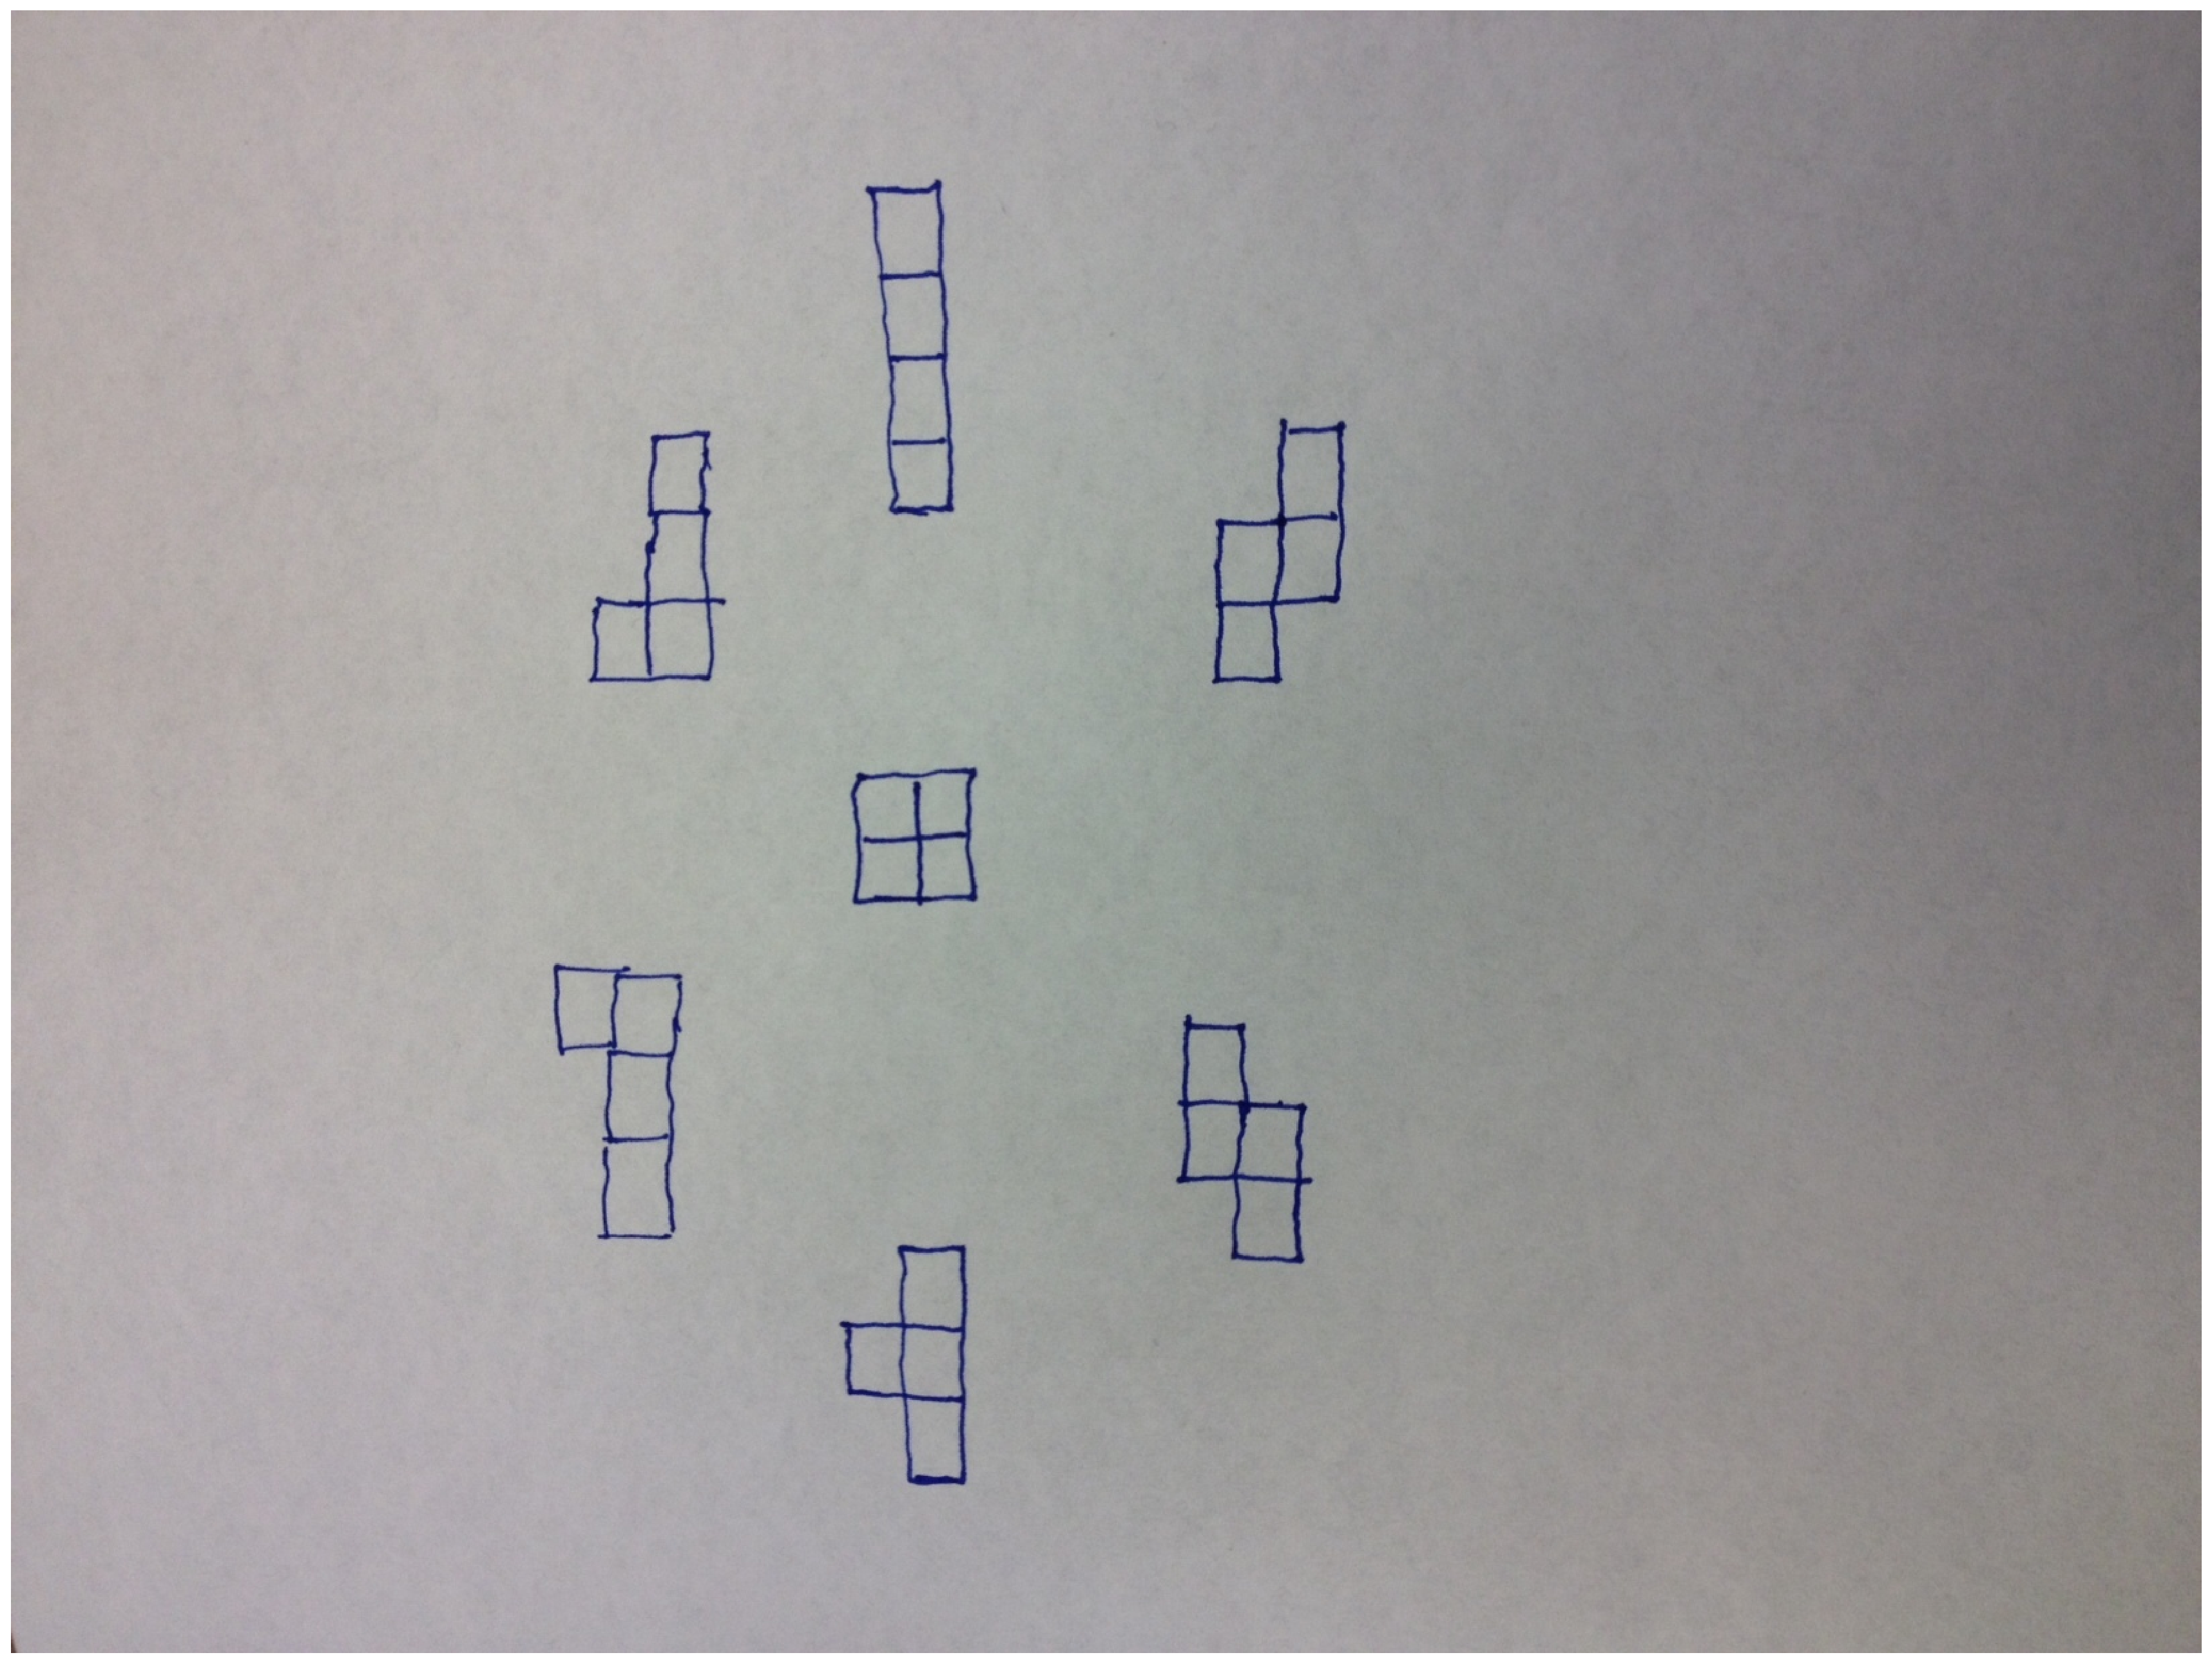
\includegraphics[scale=0.1, angle=0]{tetris.eps}
\caption{Different geometric configurations of an octahedron intermediate.}
\label{fig:OctaGCS}
\end{figure}
--embedding

\begin{mydef}
The \textbf{constraint space} corresponding to a constraint function $c: \mathbbm{R}^n \to \mathbbm{R}^{n-m}$ is its zero-set,
\begin{align}
\Omega \doteq \{z \in \mathbbm{R}^n : c(z) = 0\}.
\end{align}
\end{mydef}
If $c$ is composed of polynomial functions, then the constraint space is an algebraic variety. If this variety has no singularities, then it is also a manifold. 

Using the notion of a constraint space, we can define the space of different geometric configurations that a given intermediate can take. Since we are treating each intermediate as collection of rigid polygons attached to each other along hinged edges, there are two basic types of constraint we must enforce. First, we must ensure that the each individual face is rigid and has the correct geometric shape. Additionally, each edge to edge connection must remain fixed with only hinge-like motion allowed. 
   
\begin{mydef}
The \textbf{geometric configuration space} of a building game intermediate is a constraint space that enforces the rigidity of individual faces and hinged motion along connected edges.
\end{mydef}

To mathematically describe a particular configuration, we must specify the locations of the vertices of each face. Thus, for an intermediate $[x]$, its building game configuration space can be represented as a subset of the ambient space $\mathbb{R}^{3\times N_x}$ where $N_x \doteq \sum_{f\in x} s_f$ where $s_f$ is the number of sides (and verticies) of face $f$. Using this representation, we must then identify the corresponding constaint equations that give rise to the combinatorial configuration space as a function of points in ambient space. 

It is worth noting that while we represent each face with $3\times s_f$ coordinates, only 6 are required to speciafy a face's position and orientation if they are chosen carefully. With this in mind, we will typically use a function of $6$ of a face's vertex coordinates to constrain each of the face's remaining vertex coordinates. 


Notationally, we refer to the $k$th vertex of the $j$th face of $x$ as $v^{jk} = \left(v^{jk}_x,v^{jk}_y,v^{jk}_z\right)$.
Since the context of a constraint space requires a function $c: \mathbbm{R}^n \to \mathbbm{R}^{n-m}$, we flatten the matrix of vertex coordinates into a vector of lenghth $n = 3N_x$. 
\begin{align}
z = \begin{bmatrix} v^{1,1} \\ \vdots \\ v^{1,s_{f_1}} \\ \vdots \\ v^{|x|,1} \\ \vdots \\ v^{|x|,s_{f_{|x|}}} \end{bmatrix} \in \mathbbm{R}^n
\end{align}

There are four fundamental types of constraint equations: edge length constraints, angle constraints, and $2D$ face constraint to enforce the rigid structure of each face as well as vertex identification constraints to enforce the hinged connections.

Edge length constraints enforce that the lengths of the edges of each face in an intermediate cannot change. If the $k$th edge is definted to be that between the $(k-1)$st and $k$th vertices, we use the following function to constrain its lengths to a known value $\ell^{jk}$.
\begin{align}
c_{edge}^{j,k}\left(z\right)& = \left|v^{j,k} - v^{j,k-1}\right|^2 - (\ell_{j,k})^2 \\
& = \left(v_1^{j,k} - v_1^{j,k-1}\right)^2 +\left(v_2^{j,k} - v_2^{j,k-1}\right)^2 +\left(v_3^{j,k} - v_3^{j,k-1}\right)^2 - (\ell^{j,k})^2 
\end{align}  
This uses the notational convention that $v^{j,0} \doteq v^{j,s_j}$. For reasons that will be explained, we only explicitly enforce the lengths of two edges ($k=1,2$) per face, so there are a total of $2|x|$ edge length constraints. 

Angle constraints ensure that each face's polygonal angles are conserved. Using the dot product formula for angles, we can write this constraint as a polynomial.
\begin{align}
c_{ang}^{j,k}\left(z\right) &= (v^{j,k-1} - v^{j,k})\cdot(v^{j,k+1} - v^{j,k})  - \ell^{j,k}\ell^{j,k+1}\cos(\theta^{j,k})
\end{align}  
Here, $\theta^{j,k}$ is the angle at $v^{j,k}$ between $k$th and $(k+1)st$ edges which is a constant that is known a priori. In practice, we only enforce that the $k=1$st angle constraint for each face.

Now, between the two edge constraints and one angle constraints, we have described $3$ constraints as a function of $9$ vertex coordinates per face. Thus for any choice of the $6$ coordinates, $v^{j,1}_1, v^{j,1}_2, v^{j,1}_3, v^{j,2}_1, v^{j,2}_2, v^{j,0}_1$, the remaining $3$ coordinates, $v^{j,2}_3, v^{j,0}_2, v^{j,0}_3$, are specified by the $3$ constraint equations. Similarly, since each face's location and rotational orientation can be defined by this choice of $6$ coordinates, we have enough information to specify the coordinates of the remaining verticies. 

Since the positions of the first three verticies dictate the locations of the remaining verticies, the $2D$ face constraints use a map from the known vertex coordinates to the yet unknown locations. Using a template for what the ideal polygonal stucture for each face should be, we use a rotation matrix to specify these remaining verticies. If this template has vertices $\hat{v}^{j,0}, \hat{v}^{j,1}, \hat{v}^{j,2}, \dots, \hat{v}^{j,k}, \dots$ and the locations for $v^{j,0}, v^{j,1}, \text{and } v^{j,2}$ are known, we can identify the location of $v^{j,k}$ for $k>2$. Using this template, we can define the following length and angle constants.
\begin{align}
\ell^{j,k_1, k_2} &\doteq |\hat{v}^{j,k_1} - \hat{v}^{j,k_2}| \\ 
\phi^{j,k_1,k_2,k_3} &\doteq \cos^{-1}\left(\frac{\left(\hat{v}^{j,k_1} - \hat{v}^{j,k_2}\right)\cdot\left(\hat{v}^{j,k_3} - \hat{v}^{j,k_2}\right)}{(\ell^{j,k_1, k_2})(\ell^{j,k_3, k_2})}\right)   
\end{align}

\begin{figure}[ht]
  %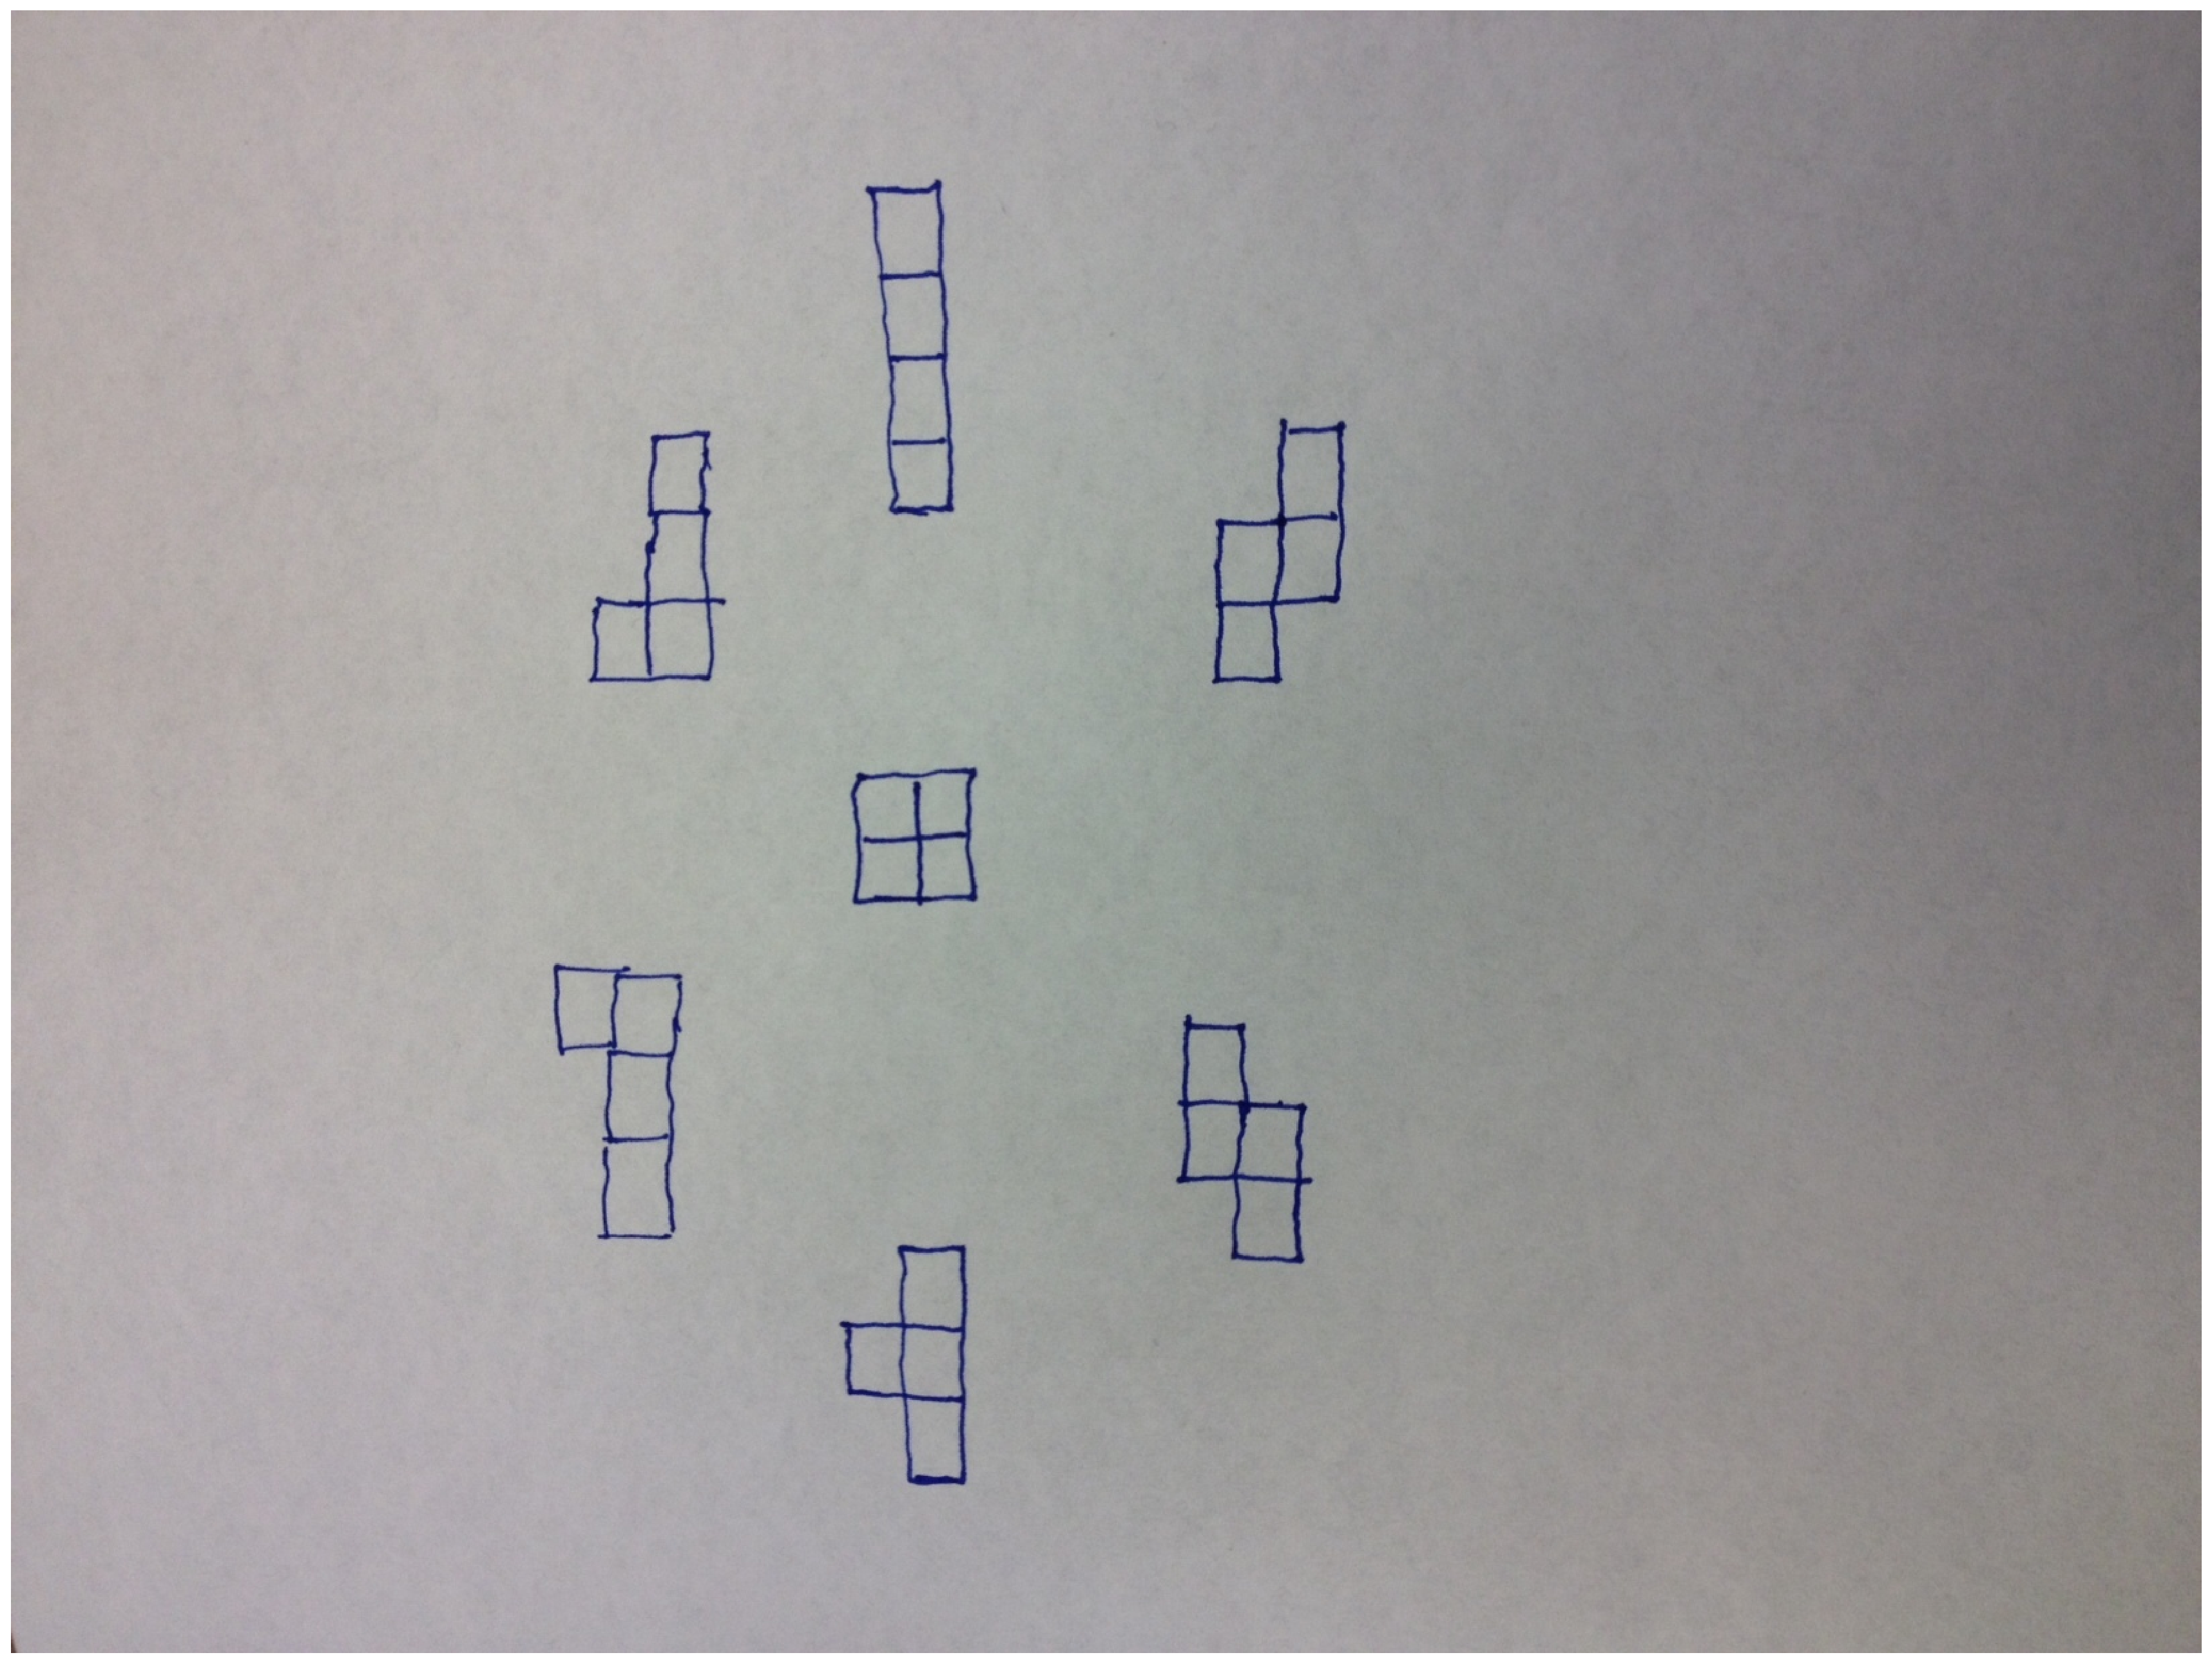
\includegraphics[scale=0.1, angle=0]{tetris.eps}
\caption{Face template and 2d face constraints.}
\label{fig:2DFC}
\end{figure}

Our basic stratigy is to first place a point $\bar{v}^{j,k}$ in the span of $v^{j,0} - v^{j,1}$ at a distance of $|\bar{v}^{j,k} - v^{j,1}| = \ell^{j,k,1}$. The choice $\bar{v}^{j,k} = v^{j,1} + \frac{\ell^{j,k,1}}{\ell^{j,0,1}}(v^{j,0} - v^{j,1})$ will work, since 
\begin{align}
  |\bar{v}^{j,k} - v^{j,1}| &= |\frac{\ell^{j,k,1}}{\ell^{j,0,1}}(v^{j,0} - v^{j,1})| \\
  &= \frac{\ell^{j,k,1}}{\ell^{j,0,1}}|v^{j,0} - v^{j,1}| \\
  &= \ell^{j,k,1}.
\end{align}
Then, a rotation matrix is used to rotate $\bar{v}^{j,k}$ by the correct angle into its position $v^{j,k}$.
The rotation matrix is centered at $v^{j,1}$ and its axis of rotation is defined by $u = \frac{1}{\ell^{j,0,1}\ell^{j,2,1}}(v^{j,0} - v^{j,1})\times(v^{j,2} - v^{j,1})$.  Similarly, the angle of rotation $\phi^{j,0,1,k}$ is the angle created by the two line segments in the template $(\hat{v}^{j,0},\hat{v}^{j,1})$ and  $(\hat{v}^{j,2},\hat{v}^{j,1})$. Thus, using $R = R(\phi^{j,0,1,k}, u)$ and our equation for $v^{j,k}$ is 
\begin{align}
v^{j,k} &= v^{1,k} + R(\bar{v}^{j,k} - v^{j,1})\\
&= v^{1,k} + \ell^{j,k,1}R(v^{j,0} - v^{j,1})\\
\end{align}
Since $R$ is polynomial in $v^{j,0}, v^{j,1}, v^{j,2}$, we get the following polynomial $2$D face constraint for each $k > 2$.
\begin{align}
c_{2D}^{j,k}(z) \doteq v^{1,k} + \ell^{j,k,1}R(v^{j,0} - v^{j,1}) - v^{j,k}
\end{align} 

The final constraint type, vertex identification, is used to enforce that the connection between edges of two faces has the mobility of a hinge. To do this, we simply need to ensure that that corresponding vertices on each edge share identical locations. This results in the relatively simple constraints:
\begin{align}
c_{ident}^{j_1,k_1,j_1,k_1,d}(z) \doteq v^{j_1,k_1}_d - v^{j_2,k_2}_d \\
\end{align}
where $v^{j_1,k_1}$ and $v^{j_2,k_2}$ are corresponding vertices from the faces $j_1$ and $j_2$ meeting at a hinged edge. If there are $|E_x|$ of these hinged connections in a building game state $x$, there must be $6|E_x|$ correcponding vertex identification constraints.

With all four constraint types explicitly defined, the aggregate constraint function for $x$ will have $n-m = 2|F_x|+ |F_x| + (N_x - 3|F_x|) + 6|E_x| = N_x + 6|E_x|$ total constraints. 


%To mathematically represent each of the possible geometric configurations, we parameterize the embedding using its vertex locations. If a building game state is composed of the faces $\{f_1,\dots, f_i\}$, then any embedding of the intermediate can be described by a point in $\mathbbm{R}^n$, where $n$ is the three times sum $3\sum_{j=1}^i \#\text{vertices}(f_j)$, of the number of vertices in each face. Simply put, the point 
% which is the concatenation of all of the vertex locations $v_1, v_2, \dots, v_{n/3} \in \mathbbm{R}^3$ for each verted on each face of an intermediate is used to represent a particular embedding. 

\subsection{Special Case of Triangular Faces}

In the case where all of the faces of the polyhedron we consider are triangles (tetrahedron, octahedron, icosahedron, etc.) we notice that by simple enforcing that each edge of each triangle has a specified length, the triangle will be rigid. This means that we do not have to use the angle and 2D face constraints. Further, rather that explicitly using vertex identification constraints, we can either treat them as length constraints with zero length between identified vertices or we can simply reindex the vertices so that identified vertices are actually treated as a single vertex. With either choice, in the trianglular case, we may only deal with length constraints if we wish. This will be a useful property in the next chapter. 

Additionally, we make a conjecture that under certain trianglular conditions, our algebraic variety has no singularities and is thus a manifold.
\begin{mycon}
\label{con:TriMan}
The geometric configuration space for each intermediate composed of equilateral triangular faces is a manifold.
\end{mycon}

\section{Degrees of Freedom}
Roughly speeking, the degrees of freedom of a system are the different independent motions the system is able to exercise. Since the concept of degrees of freedom exists in many diverse scientific fields, such as mechanical engineering and statistical physics, many different formal definitions of degrees of freedom are used in the literature~\cite{Pennestri2005}. McCarthy defines degrees of freedom of a mechanical system as follows~\cite{McCarthy1990}. 
\begin{quote}
We derive formulas for the number of parameters needed to specify the configuration of a mechanism, in terms of the number of links and joints and the freedom of movement allowed at each joint. This number is the \textit{degrees of freedom} or \textit{mobility} of the mechanism. Changing the values of these parameters changes the configuration of the mechanism. Thus, if we view the set of all configuration available to a mechanism as a manifold, then the mobility of the mechanism is the dimension of this manifold. 
\end{quote}

Since our geometric configuration space is an algebraic variety and not a manifold in general, this definition must be modified to make degrees of freedom a statistic of each individual configuration rather than a global statistic of the geometric configuration space. 

\begin{mydef}
The number of \textbf{degrees of freedom} a building game intermediate at configuration $z$ is the dimension of the geometric configuration space algebraic variety at $z$. If $z$ is a singularity of the algebraic variety, then the degrees of freedom is undefined.
\end{mydef}

In most cases we consider, rigid rotation and rigid translation will preserve the value of the constraint function since they do not move the verticies relative to one another. In other words, if $c(z) = 0$ then we also have $c(Rz + T) = 0$ where $R \in \mathbbm{R}^{n}\times n$ rotates each vertex in the configuration by some $\hat{R} \in SO(3)$ and translates each vertex by $\hat{T} \in \mathbbm{R}^3$. With this definition, $R$ is the block diagonal matrix with each of the $n/3$ block being $\hat{R} \in SO(3)$ and $T \in \mathbbm{R}^n$ is composed of $n/3$ copies of $\hat{T} \in \mathbbm{R}^3$ stacked upon each other. These rigid body rotations account for $6$ of the configuration's degrees of freedom: $3$ rotational degrees of freedom and $3$ translational.
\begin{mydef}
The \textbf{trivial degrees of freedom} a building game intermediate at configuration $z$ are the $6$ degrees of freedom corresponding to rigid body rotations and translations.
\end{mydef}
Thus, the degrees of freedom we are most interested in are those that do represent movement of the verticies and faces relative to each other. 
\begin{mydef}
The \textbf{internal degrees of freedom} a building game intermediate at configuration $z$ are the degrees of freedom that are not trival.
\end{mydef}

\subsection{Computing Degrees of Freedom}

For a general constraint space, we can find the dimension of the space at a point $z$ by looking at the Jacobian matrix $C(z) \in \mathbbm{R}^{(n-m)\times n}$ of the constraint function $c$. Since the number of degrees of freedom is defined to be the dimension of that space, we look at the rank of the Jacobian. Since this rank quantifies the number of independent constraints given by $c$ at $z$, the number of degrees of freedom is given by the following.
\begin{align}
DoF &\doteq n - \text{rank}\left((C(z)\right)
\end{align}
Since the rank can take values between $0$ and $\min\{n,n-m\} = n-m$, there can be anywhere from $0$ degrees of freedom, when there are functionally no constraints on $z$, and $m$ degrees of freedom in the case where all $n-m$ constraint equations are independent and $C(z)$ is of full rank. 

In the typical case in which the constraint equations are invarient under three-dimensional rotation and translation, there will be six trivial degrees of freedom. The number of internal degrees of freedom would then be $n - \text{rank}\left((C(z)\right) - 6$.  

\begin{mydef}
If there are zero iternal degrees of freedom at a onfiguration $z$, we say that the configuration is \textbf{rigid}.
\end{mydef}

To actually compute the number of degrees of freedom for configurations of building game intermediates, we must first find an explicit form for the Jacobian matrix $C$. Below are the partial derivatives of the constraint functions we specified above.  
\begin{align}
	\frac{\partial c_{edge}^{j,k}}{\partial z_i} &=
  	\begin{cases}
        	2\left(v^{j,k}_d-v^{j,k-1}_d\right) 	& \text{if } z_i = v^{j,k}_d \\
   		-2\left(v^{j,k}_d-v^{j,k-1}_d\right) 	& \text{if } z_i = v^{j,k-1}_d \\
   		0       				& \text{else} 
  	\end{cases} \\
	\frac{\partial c_{ang}^{j,k}}{\partial z_i} &=
  	\begin{cases}
        	v^{j,k+1}_d-v^{j,k}_d 			& \text{if } z_i = v^{j,k-1}_d \\
        	2v^{j,k}_d-v^{j,k-1}_d -v^{j,k+1}_d 	& \text{if } z_i = v^{j,k}_d \\
   		v^{j,k-1}_d-v^{j,k}_d 			& \text{if } z_i = v^{j,k+1}_d \\
   		0       				& \text{else} 
  	\end{cases} \\
	\frac{\partial c_{2D}^{j,k}}{\partial z_i} &=
  	\begin{cases}
        		& \text{if } z_i = v^{j,0}_d \\
        		& \text{if } z_i = v^{j,1}_d \\
        		& \text{if } z_i = v^{j,2}_d \\
          	-1 	& \text{if } z_i = v^{j,k}_d \\
   	  	0 	& \text{else} 
  	\end{cases} \\
	\frac{\partial c_{ident}^{j_1,k_1,j_2,k_2,d}}{\partial z_i} &=
  	\begin{cases}
        	1 	& \text{if } z_i = v^{j_1,k_1}_d \\
        	-1 	& \text{if } z_i = v^{j_2,k_2}_d \\
   		0       & \text{else} 
  	\end{cases} 
\end{align}

Since the number of degrees of freedom is defined as a local property of a specific configuration $z$, different configurations of the same building game intermediate could theoretically have differing numbers of degrees of freedom. However, we have yet to observe a building game intermediate that has this property and is evidence that supports conjecture~\ref{con:TriMan}. A contrived case in which a linkage of squares leads to a configuration space with differing degrees of freedon is described in section~\ref{ssc:NonMan}. When we report the number of degrees of freedom that a building game intermediate has, we use its connonical configuration in computation.
\begin{mydef}
The \textbf{cannonical configuraion} of a building game intermediate $[x]$ is the configuration that is simply the $3$-dimensional embedding of the polyhedron restricted to the faces in $x$
\end{mydef}
For example, in the case of the cube, the cannonical configuration would have all of the faces of the intermediate  meeting at right angles just as they do in the cube itself. 

In practice, we use NumPy's numpy.linalg.svd module to take the singlular value decomposition of the compute Jacobian matrix in Python. The rank of the Jacobian is then the number of effectively non-zero singlular values where a small cutoff is used to determine whether a small singular value is indeed zero or non-zero.

\subsection{Non-Manifold Example}
\label{ssc:NonMan}
%From this definition, it is worth noting that if the geometric configuration space is indeed a manifold, then the degrees of freedom is the dimension of that manifold which is a global property. Here we present an interesting example in which this is not the case and, depending on the specific configuration, a different number of degrees of freedom exist.

Consider the linkage of six squares aranged in a $2\times 3$ lattice depicted in figure~\ref{fig:SixSq}. This linkage has three lines of hinges: 2 accross and 1 down. As shown, the two horizontal hinges can be manipulated independently with each of the vertical hinges maintaining at an angle of $\pi$ degrees. This seems to indicate two internal degrees of freedom. Alternatively, when folded along the verticle crease, the horizontal hinges remain fixed with dihedral angle $\pi$. This configuration corresponds to just a single internal degree of freedom. Thus, the transition between these two modes, when the linkage is completely planar, there is a singularity and the number of degrees of freedom is not definied. 

\begin{figure}[ht]
  %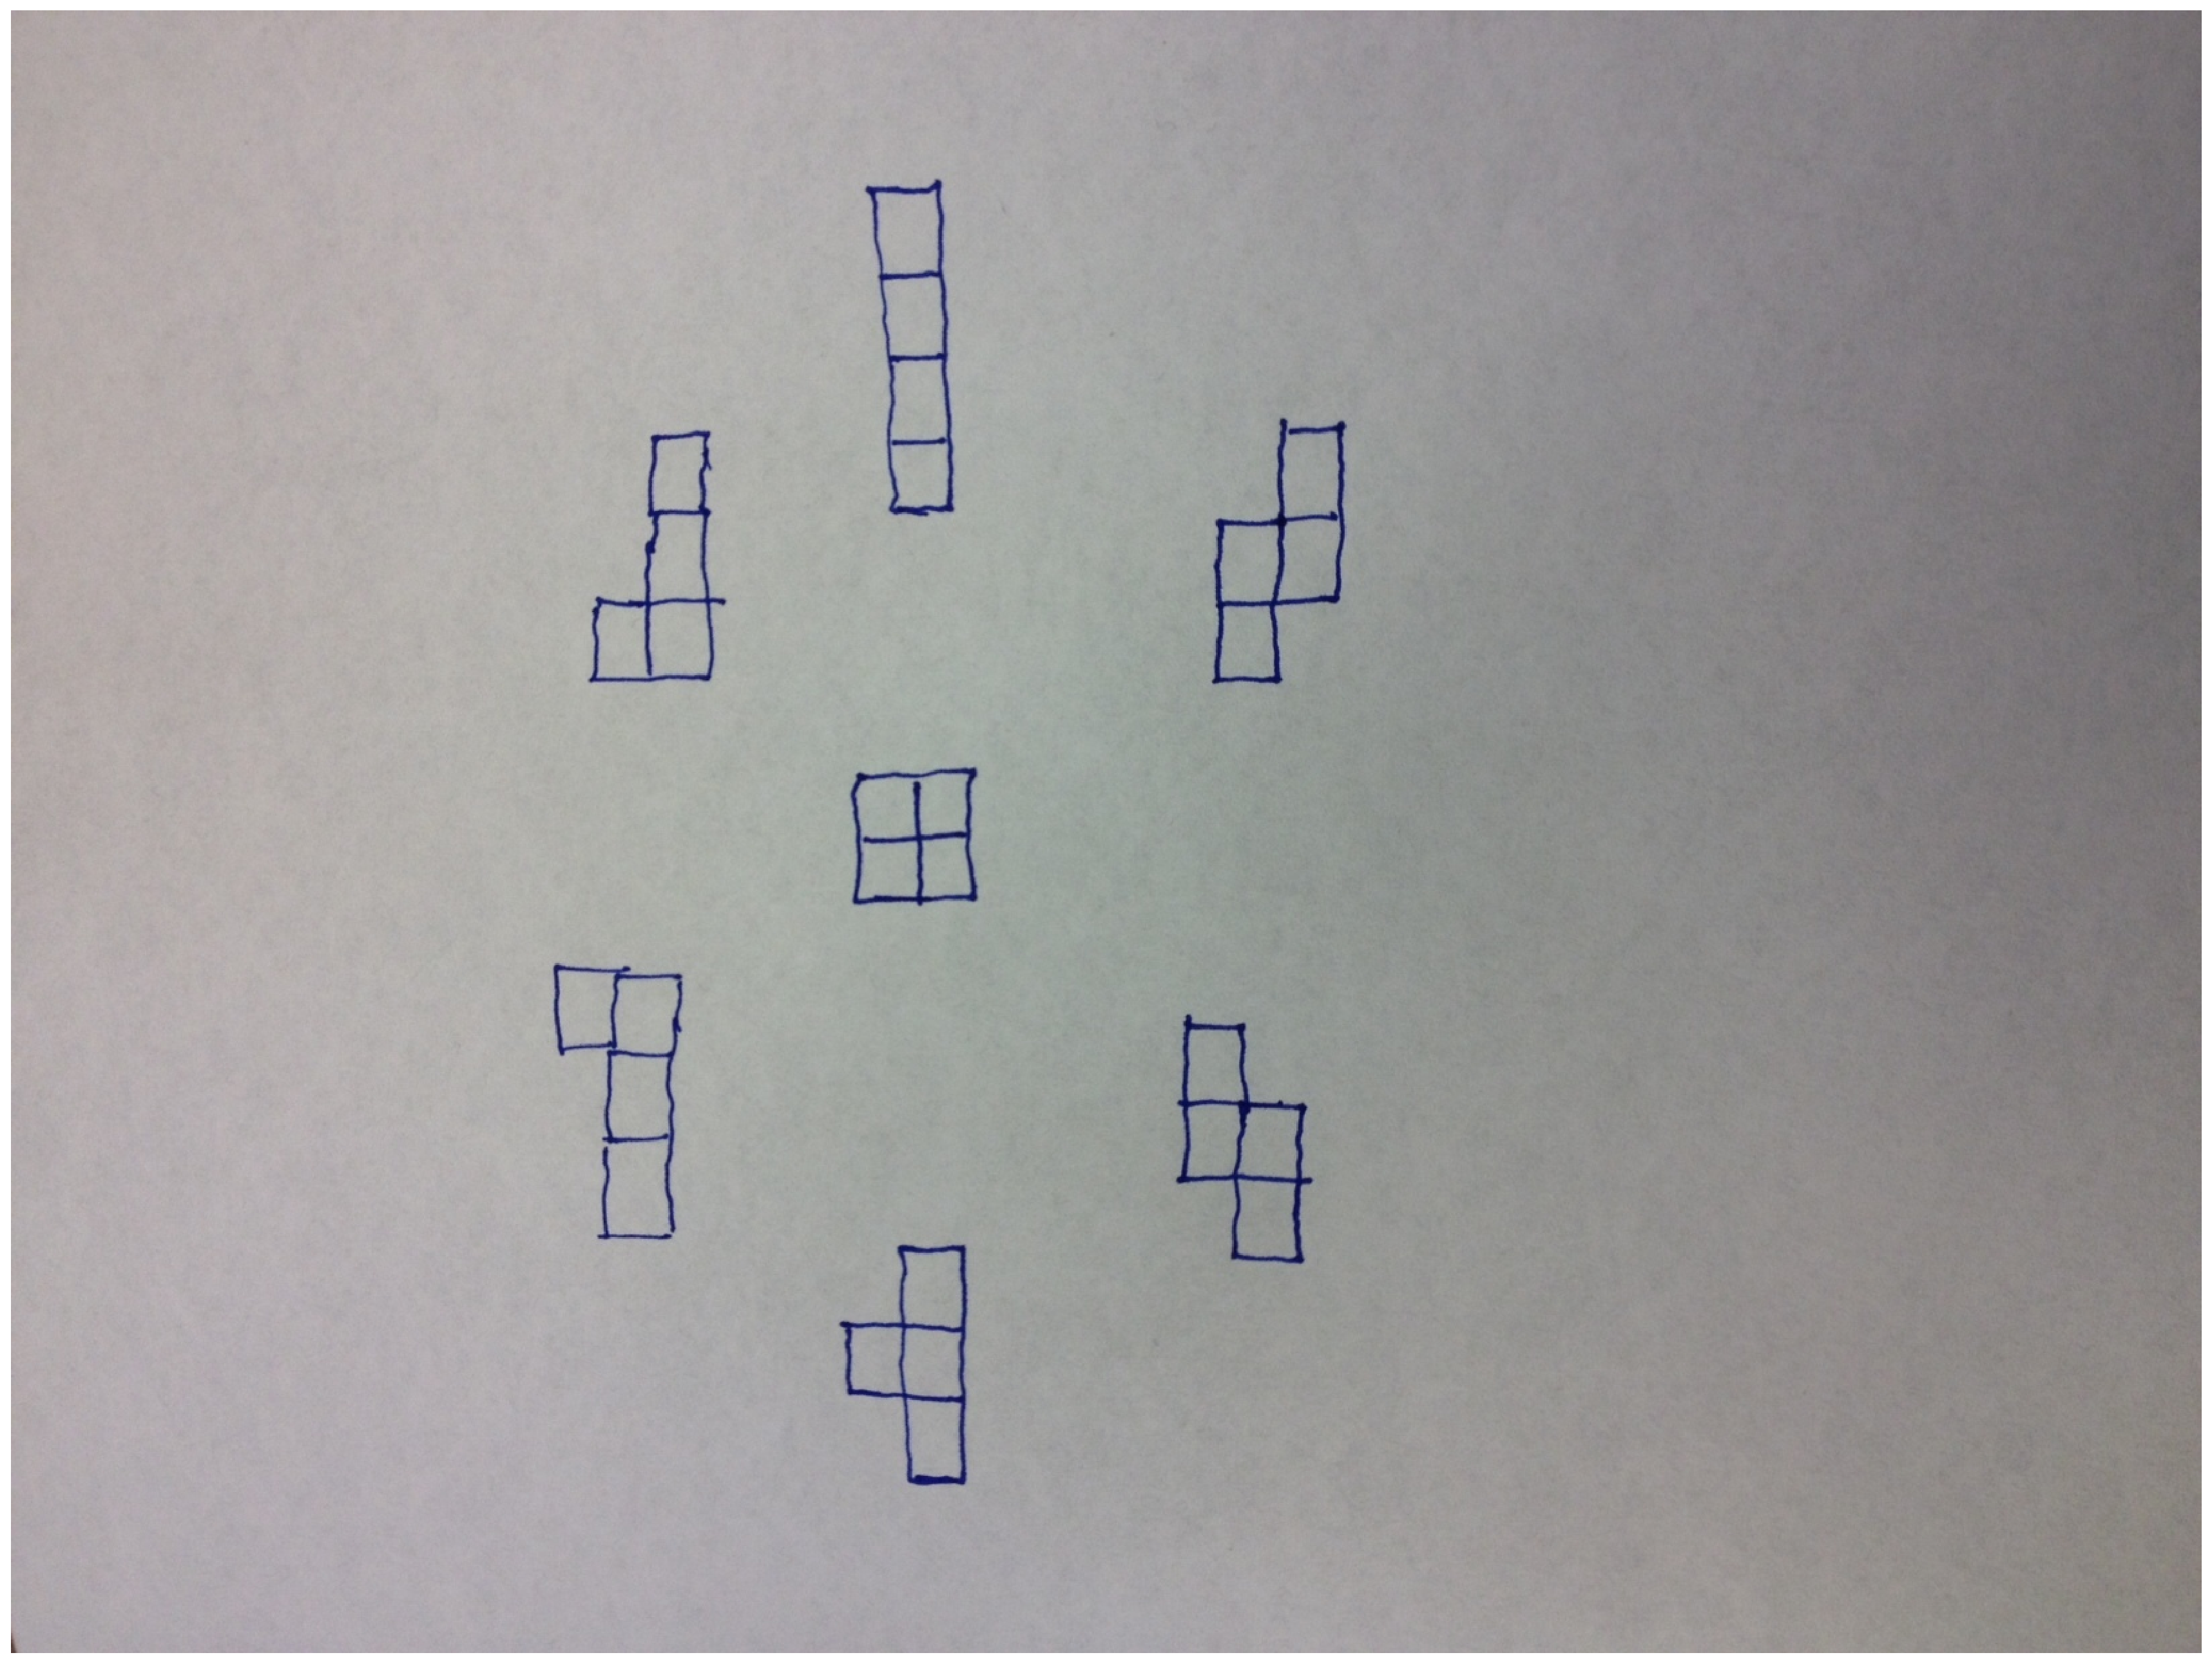
\includegraphics[scale=0.1, angle=0]{tetris.eps}
\caption{A linkage of 6 squares with configurations of different degrees of freedom.}
\label{fig:SixSq}
\end{figure}

As stated previously, we have not observed this type of behavior from any building game intermediates. This leads us to speculate that the degenerate nature of this example is down to an uncommon alignment of the hinged edges. Clearly, this linkage could never be an intermediate of a convex polyhedron. Perhaps the building game geometric configuration space has no singularities and is hence a manifold for all convex polyhedra.  

\subsection{Results}


\begin{figure}[ht]
\centering
  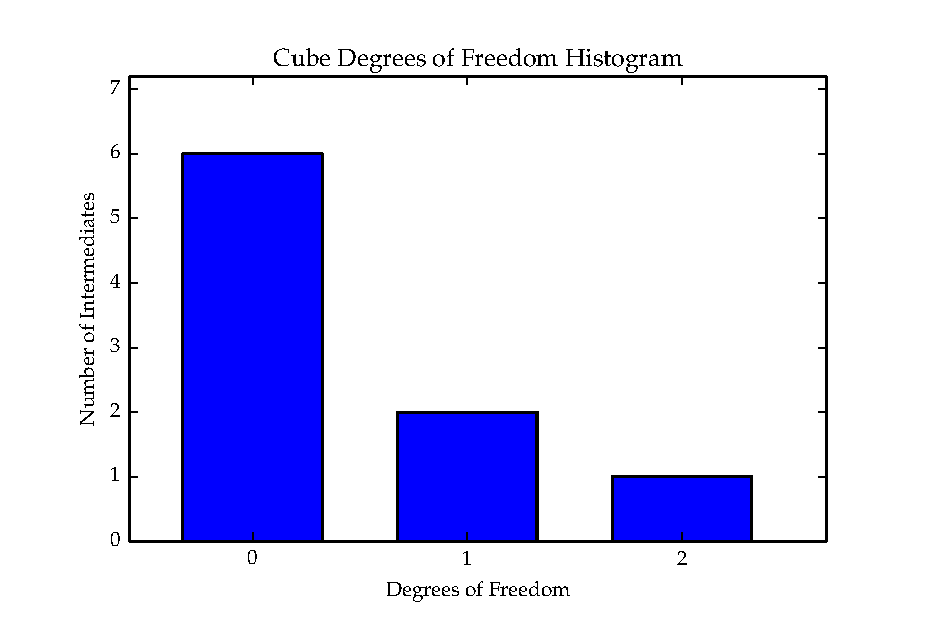
\includegraphics[scale=1.0, angle=0]{cube_dof_hist.eps}
\caption{Distribution of internal degrees of freedom amongst Cube intermediates.}
\label{fig:CubeDoFHist}
\end{figure}

\begin{figure}[ht]
\centering
  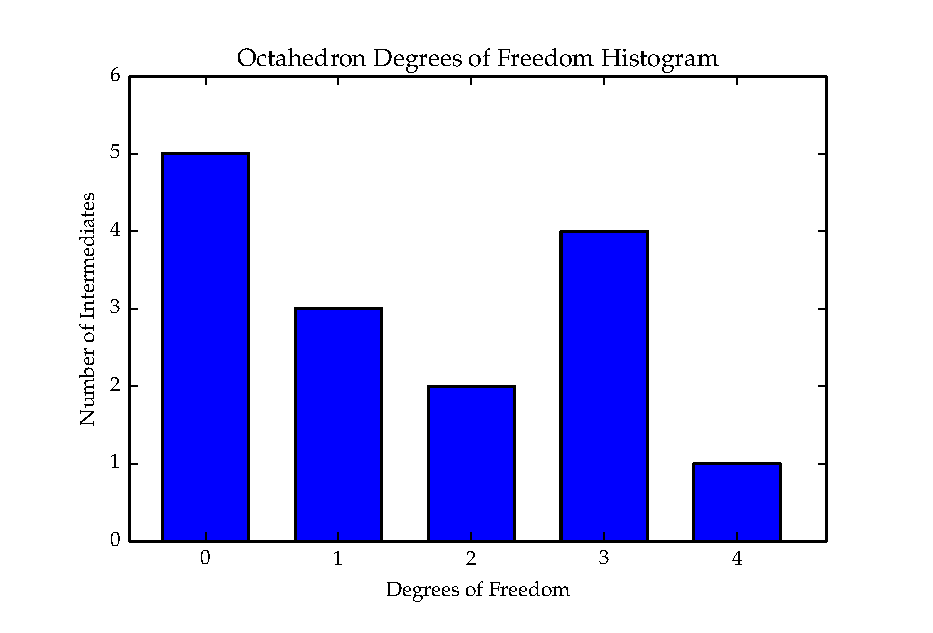
\includegraphics[scale=1.0, angle=0]{octahedron_dof_hist.eps}
\caption{Distribution of internal degrees of freedom amongst Octahedron intermediates.}
\label{fig:OctaDoFHist}
\end{figure}

\begin{figure}[ht]
\centering
  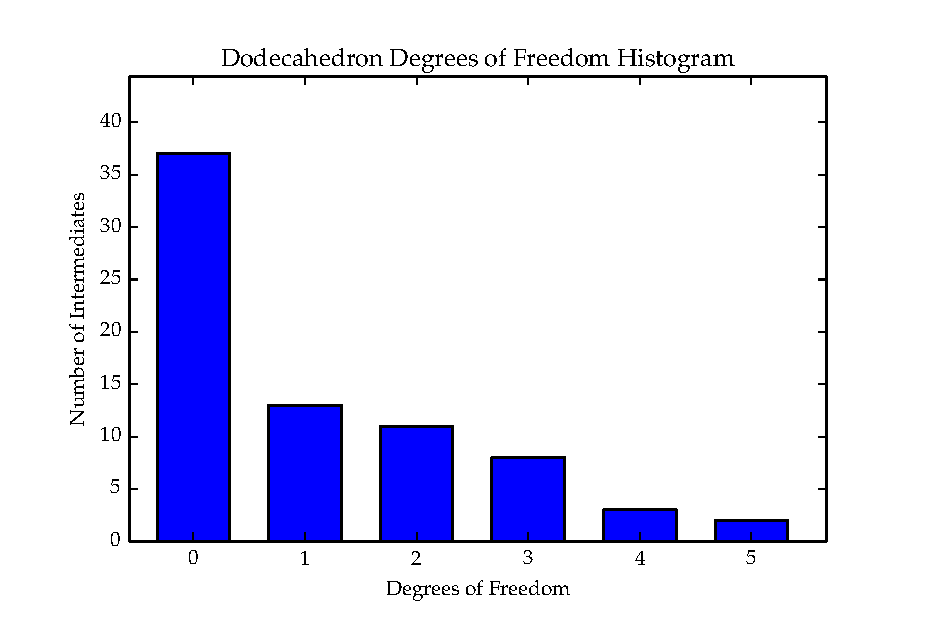
\includegraphics[scale=1.0, angle=0]{dodecahedron_dof_hist.eps}
\caption{Distribution of internal degrees of freedom amongst Dodecahedron intermediates.}
\label{fig:DodecDoFHist}
\end{figure}

\begin{figure}[ht]
\centering
  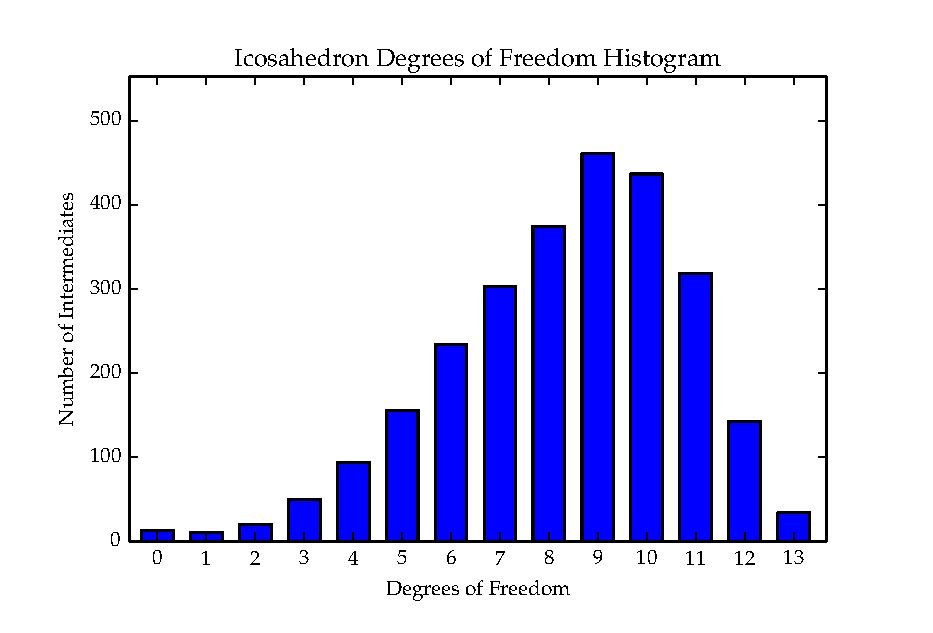
\includegraphics[scale=1.0, angle=0]{icosahedron_dof_hist.eps}
\caption{Distribution of internal degrees of freedom amongst Icosahedron intermediates.}
\label{fig:IcosaDoFHist}
\end{figure}

Using the Jacobian method for computing internal degrees of freedom, we have computed the number of degrees of freedom for all intermediates of the Platonic solids. Figures~\ref{fig:CubeDoFHist},~\ref{fig:OctaDoFHist},~\ref{fig:DodecDoFHist}, and~\ref{fig:IcosaDoFHist} are histograms of the number of internal degrees of freedom for the intermediates of each of the Platonic solids. We do not include the Tetrahedron, since it only has four intermediates and only the one composed of two triangles is not rigid. Interestingly, the cube and dodecahedron have a large number of rigid intermediates due  to the fact that their verticies are the rigid meeting of only three faces. The octahedron, with four faces meeting at each vertex has a more varied distribution of internal degrees of freedom. The icosahedron, however, has a very small number of rigid intermediates with some intermediates having as many as $13$ internal degrees of freedom. 

\begin{figure}[ht]
\centering
  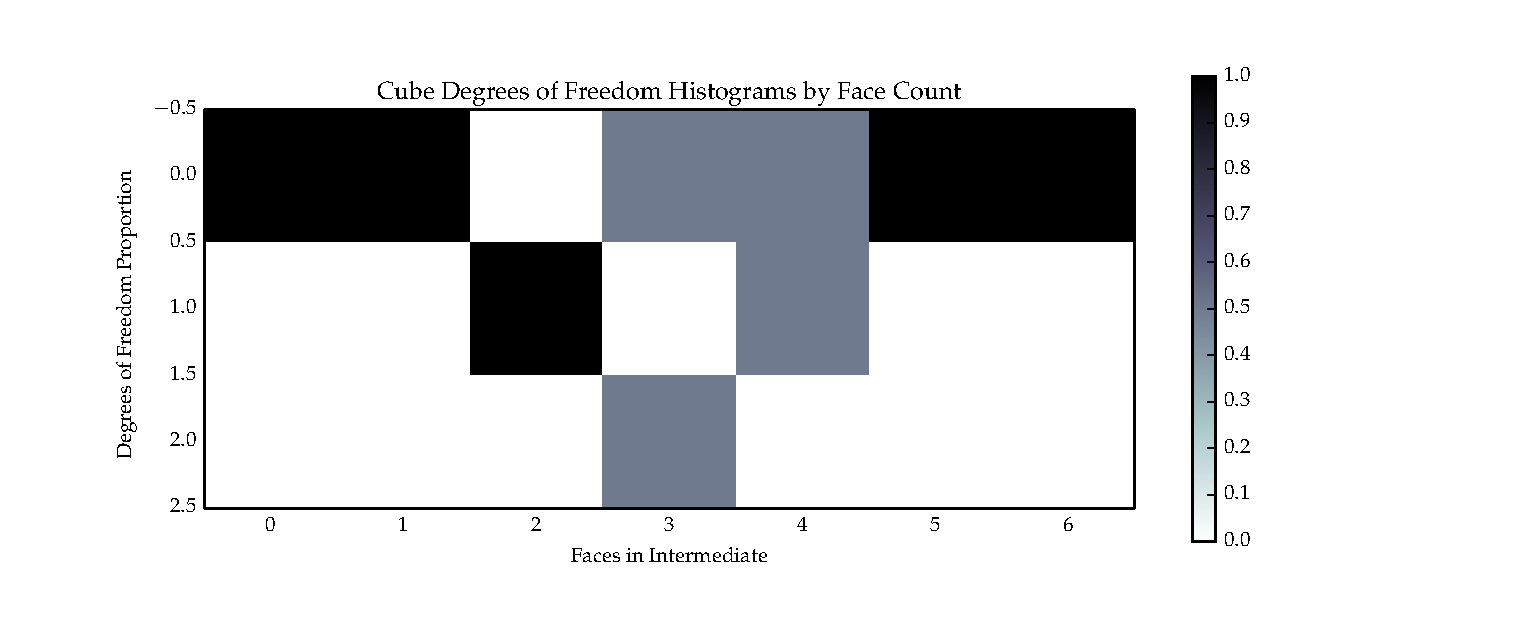
\includegraphics[scale=0.7, angle=0]{cube_dof_hist_facecount.eps}
\caption{Each virtical column gives a histogram of the number of internal degrees of freedom $k$-faced intermediates of the cube have.}
\label{fig:CubeDoFHistFC}
\end{figure}

\begin{figure}[ht]
\centering
  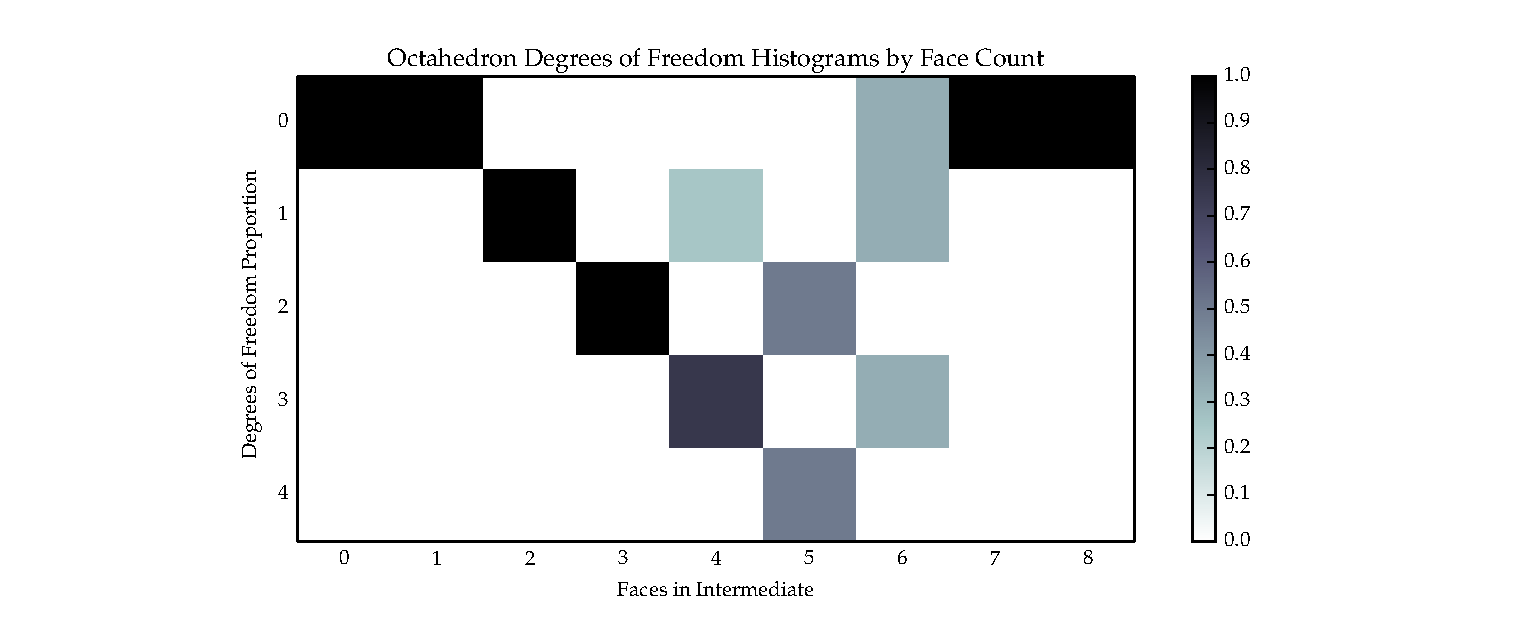
\includegraphics[scale=0.7, angle=0]{octahedron_dof_hist_facecount.eps}
\caption{Each virtical column gives a histogram of the number of internal degrees of freedom $k$-faced intermediates of Octahedron have.}
\label{fig:OctaDoFHistFC}
\end{figure}

\begin{figure}[ht]
\centering
  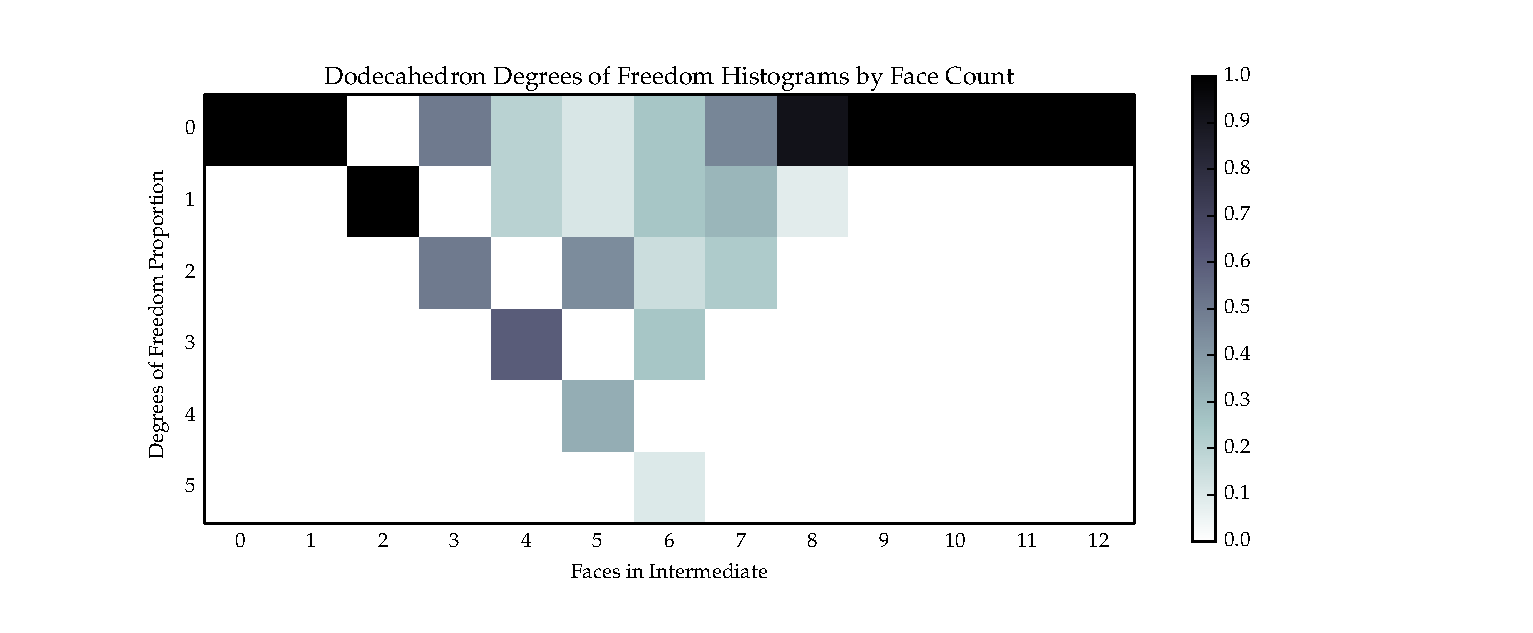
\includegraphics[scale=0.65, angle=0]{dodecahedron_dof_hist_facecount.eps}
\caption{Each virtical column gives a histogram of the number of internal degrees of freedom $k$-faced intermediates of the Dodecahedron have.}
\label{fig:DodecDoFHistFC}
\end{figure}

\begin{figure}[ht]
\centering
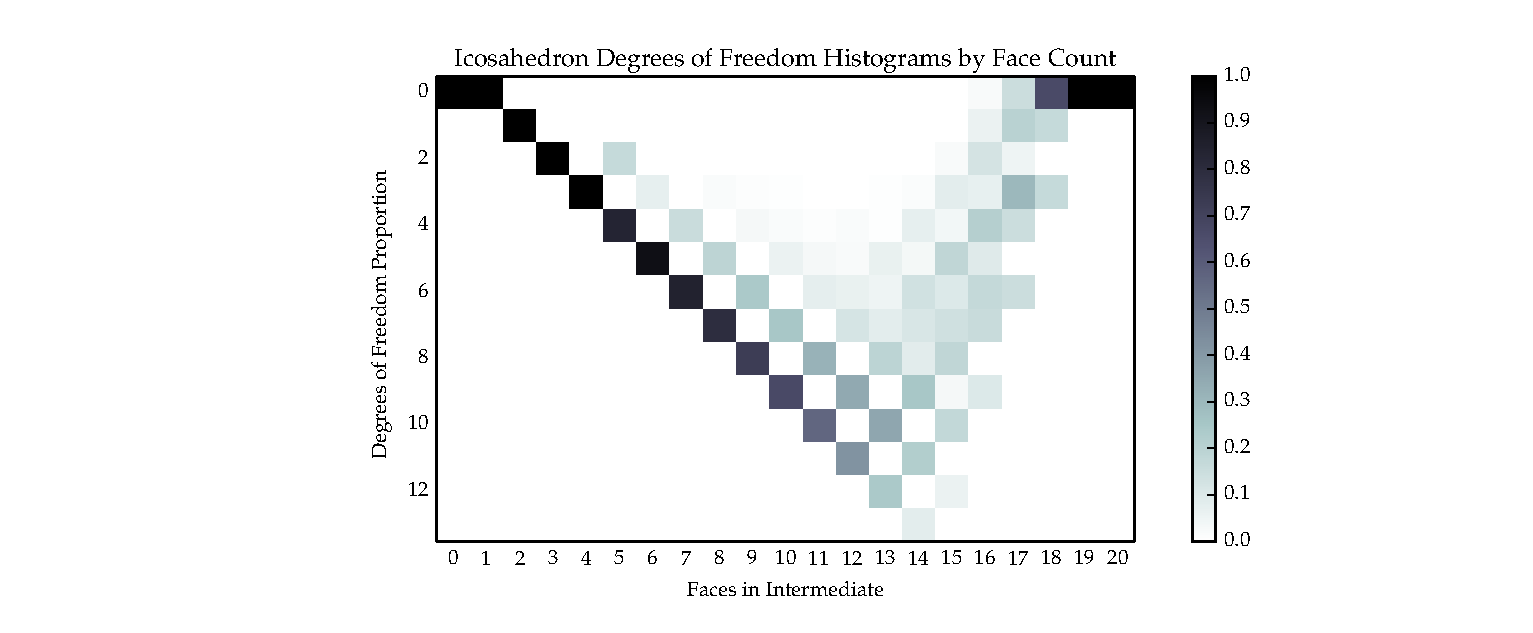
\includegraphics[scale=0.7, angle=0]{icosahedron_dof_hist_facecount.eps}
\caption{Each virtical column gives a histogram of the number of internal degrees of freedom $k$-faced intermediates of the icosahedron have.}
\label{fig:IcosaDoFHistFC}
\end{figure}

To provide a more detailed look at the distribution of internal degrees of freedom, figures~\ref{fig:CubeDoFHistFC},~\ref{fig:OctaDoFHistFC},~\ref{fig:DodecDoFHistFC}, and~\ref{fig:IcosaDoFHistFC} break down the previous histograms by the number of faces in the intermediate. Each column of the plots is a histogram for the number of internal degrees of freedom for the intermediates with that specific number of faces. The general theme seems to be that intermidiates with almost all or almost none of their faces are most rigid and the intermediates with around half of the total possible faces have the most internal degrees of freedom. The most interesting case remains the icosaheron with a wide variation in internal degrees of freedom for most face counts.

\subsection{Explicit Removal of Trivial Degrees of Freedom}
\label{ssc:RemTrivDoF}
Since we are often solely interested the internal degrees of freedom, there are a few was to augment the constraint equations to mod out the translation or rotations causing the trivial degrees of freedom. One possible choice is to pick a face and constrain its vertex locations to match a fixed template. The corresponding constraint equations for fixing the $j$th face would be
\begin{align}
c_{fix}^{j,k,d}\left(z\right) &= v^{j,k}_d - \hat{v}^{j,k}_d \\
	\frac{\partial c_{fix}^{j,k,d}}{\partial z_i} &=
  	\begin{cases}
        	1 	& \text{if } z_i = v^{j,k}_d \\
   		0       & \text{else} 
  	\end{cases} 
\end{align}
for each dimension $d$ of each vertex $k$ of face $j$. For reasons we will explain in the next chapter, this may not always be an ideal choice if there is information other than the degrees of freedom we wich to derive from the constraint equations.


An alternative that prevents translation, but does allow rotation is to fix the configuration's center of mass. 
\begin{align}
c_{com}^{d}\left(z\right) &= \sum_{j = 1}^{|F_x|}\sum_{k=1}^{s_{f_j}}v^{j,k}_d \\
	\frac{\partial c_{com}^{d}}{\partial z_i} &=
  	\begin{cases}
        	1 	& \text{if } z_i = v^{j,k}_d \\
   		0       & \text{else} 
  	\end{cases} 
\end{align}
This amounts to the sum over the $d$th entry of each vertex in the configuration.

%We consider the linkage of rigid 2-dimensional polygons in $\mathbb{R}^3$ by means of ideal hinges located at the edges of the polygons. In this way, by treating intermediates of our various models as such a linkage, we can compute the non-trivial degrees of freedom (DoF) each intermediate has. 

%Every linkage of this type has 6 trivial degrees of freedom: 3 corresponding to translational movement and 3 corresponding to rotational freedom. While these freedoms do change the orientation of the intermediate, they do not cause the faces to move relative to each other. For this reason, we label them as trivial degrees of freedom and focus on the calculation the remaining, non-trivial degrees of freedom. 

%For our purposes, we define the \textbf{degrees of freedom} of a configuration to be the difference between the number of parameters needed to specify a configuration in an ambient parameter space $\Omega$ and the number of independent constraints imposed upon the configuration as a function of these parameters. Consequently, the non-trivial degrees of freedom is the number of degrees of freedom minus the six trivial degrees of freedom. If the ambiant parameter space is $\mathbb{R}^N$ and there are $M$ constraint equations given by $\varphi : \mathbb{R}^N \to \mathbb{R}^M$, we find the degrees of freedom to be $N - \operatorname{rank}(\varphi)$ and the non-trivial degrees of freedom to be $N - \operatorname{rank}(\varphi) - 6$. Here we need $\varphi$ to be a smooth map so that the rank is well defined. Furthermore, we define the \textbf{configuration space} to be the subset of parameter space $\{\omega \in \Omega : \varphi(\omega) = 0\}$ upon which the contraints are satisfied.


%In our case, the location and orientation of each polygon in the linkage can be represented by a total of 6 parameters: 3 for location and 3 for roational orientation. Thus, the entire configuration of an intermediate $x$ can be represented in the parameter space $\mathbb{R}^{F_x\times6}$. With constraints corresponding to hinged connections we construct a function $\varphi$ which is zero if and only if the constraints are satisfied. Thus the configuration space is $\{z \in \mathbb{R}^{F_x\times6} : \varphi(z) =0\}$. As we will show below, the constraint equation $\varphi$ can be constructed as a polynomial which means that the configuration space (as the zero set of this polynomial) is an algebraic variety. 

% PARAGRAPH ON DIFFERENT DOF VALS AT DIFFERENT CONFIGS OF SAME INTERMEDIATE We refer to the embedded configuration of $x$ such that $x$ is a subset of the original polyhedron as the \textbf{canonical configuration}.


%The base constaints are put in place to fix one of the intermediate's faces in space to remove the 6 trivial degrees of freedom from the calculation. If $f_b$ is the face we wish to designate as the base we have the following $3\times s_b$ constraint equations
%\begin{align}
%\psi_{base}^{k,x}\left(\mathbf{v}\right)& = v^{b,k}_x - c^{b,k}_x \\
%\psi_{base}^{k,y}\left(\mathbf{v}\right)& = v^{b,k}_y - c^{b,k}_y \\
%\psi_{base}^{k,z}\left(\mathbf{v}\right)& = v^{b,k}_z - c^{b,k}_z
%\end{align}  
%for $k = 1,\dots,s_b$ and with $c^{b,k}_\bullet$ a known constant. The corresponding Jacobian calculation for each constraint equations is:
%\[
%\frac{\partial\psi_{base}^{k,\bullet}}{\partial v} =
%  \begin{cases}
%   1 & \text{if } v = v^{b,k}_\bullet \\
%   0       & \text{else} 
%  \end{cases}
%\]

%Edge length constraints enforce that the lengths of the edges of each face in an intermediate cannot change. Since there are $s_j$ edges for each face $f_j$ of intermediate $x$, there are $N_x$ corresponsing edge constraints. 
%\begin{align}
%\psi_{edge}^{j,k}\left(\mathbf{v}\right)& = \left|v^{j,k} - v^{j,k-1}\right|^2 - \ell_{j,k}^2 \\
%& = \left(v_x^{j,k} - v_x^{j,k-1}\right)^2 +\left(v_y^{j,k} - v_y^{j,k-1}\right)^2 +\left(v_z^{j,k} - v_z^{j,k-1}\right)^2 - \ell_{j,k}^2 
%\end{align}  
%for all $j: f_j \subset x$ and with the convention that $v^{j,0} \doteq v^{j,s_j}$ and $\ell_{j,k}$ is a known constant. The resulting partial derivatives are
%\[
%	\frac{\partial\psi_{edge}^{j,k}}{\partial v} =
%  	\begin{cases}
%        	2\left(v^{j,k}_\bullet-v^{j,k-1}_\bullet\right) 	& \text{if } v = v^{j,k}_\bullet \\
%   		-2\left(v^{j,k}_\bullet-v^{j,k-1}_\bullet\right) 	& \text{if } v = v^{j,k-1}_\bullet \\
%   		0       & \text{else} 
%  	\end{cases}
%\]
%--definiteion of 'base configuration'
%--representation of config space definition as system of constraint equations
%--solution of the constraint equations is a manifold except perhaps at some 'sp0ecial' configurations
%--define DoF as 6N - rank of the jacobian of the CEqs evaluated at the base config

%--go through computation of jacobian  




%\section{Cyclohexane Application}
%??Include??
%\subsection{Sachse Model}
%
%Around the turn of the century, it was thought that cyclohexane's carbon atoms must lie in a plane. A young German assistant, Hermann Sachse, had the idea that allowing the carbons to lie outside the plan could alleviate the angle strain. Inspired by polyhedral geometry, he templates and outlined methods for creating 3D models of the chair and boat configurations his new theory conceptualized. Figure~\ref{fig:sachse} shows a construction of these two models. Despite his best efforts, Sachse's ideas were not accepted by that chemistry community until after his death. 
%
%
%
%\begin{figure}
%        %\centering
%        %\begin{subfigure}[b]{0.24\textwidth}
%        %        \includegraphics[width=\textwidth]{chair_model_2.png}
%        %        \caption{Chair (top)}
%        %        \label{fig:CM1}
%        %\end{subfigure}%
%        %~ %add desired spacing between images, e. g. ~, \quad, \qquad etc.
%        %  %(or a blank line to force the subfigure onto a new line)
%        %\begin{subfigure}[b]{0.24\textwidth}
%        %        \includegraphics[width=\textwidth]{chair_model_1.png}
%        %        \caption{Chair (side)}
%        %        \label{fig:CM2}
%        %\end{subfigure}%
%        %~ %add desired spacing between images, e. g. ~, \quad, \qquad etc.
%        %  %(or a blank line to force the subfigure onto a new line)
%        %\begin{subfigure}[b]{0.24\textwidth}
%        %        \includegraphics[width=\textwidth]{boat_model_1.png}
%        %        \caption{Boat (top)}
%        %        \label{fig:BM1}
%        %\end{subfigure}%
%        %~ %add desired spacing between images, e. g. ~, \quad, \qquad etc.
%        %  %(or a blank line to force the subfigure onto a new line)
%        %\begin{subfigure}[b]{0.24\textwidth}
%        %        \includegraphics[width=\textwidth]{boat_model_2.png}
%        %        \caption{Boat (side)}
%        %        \label{fig:BM2}
%        %\end{subfigure}%
%        %\caption{Sachse Models}\label{fig:sachse}
%\end{figure}
%
% 
%\subsection{Idealized Constraint Model}\label{building_game}
%
%Withe the eclipsing and angle strains in mind, we heuristically define an idealized model of cyclohexane by imposing geometric constraints. Each configuration is represented by the 3-dimensional locations of the center of its carbon atoms and we explicitly parameterize these locations as $v_1, v_2, \dots, v_6$ where $v_k \in \mathbb{R}^3$. For ease of exposition, $v_0 \doteq v_6$ and $v_{-1} \doteq v_5$ are notationally identified. 
%
%First, we require that any two atoms sharing a bond have a known and fixed distance $\ell$ from each other. Since we can re-scale our coordinate system, we assume $\ell \doteq 1$. Additionally, we assume that the connectivity of the cyclohexane molecule is such that $v_k$ is bonded to $v_{k-1}$ for $k = 1,\dots,6$. This gives our first six constraint equations.
%$$0 = \varphi_{len}^k\left(v_{k-1},v_{k}\right) = \|v_k-v_{k-1}\| - 1 $$
%for $k = 1,\dots,6$. 
%
%Additionally, we impose constraints representing the angle strain. Since the carbon atoms have the lowest energy when their bonds are at tetrahedral angles, we fix the angle of each set of three adjacent carbons to be at the tetrahedral angle. This is equivalent to the six angle constraint equations 
%$$0 = \phi_{ang}^k\left(v_{k-2},v_{k-1},v_{k}\right) = \left(v_k-v_{k-1}\right)\cdot \left(v_{k-2}-v_{k-1}\right) + \frac{1}{3}$$
%for $k = 1,\dots,6$.
%
%\subsection{Degrees of Freedom in Ideal Model}
%
%The first step in answering these questions is determining whether there is any degrees of freedom to each configuration or whether they are rigid. This can be determined by using established theory on rigidity of linkages and degrees of freedom. By computing the Jacobian matrix $J(v)$ of the system of constraint equations, we have the following equation for the degrees of freedom for a constraint satisfying set of coordinates $v$.
%$$DoF(v) = 18 - rank(J(v))$$
%When the Jacobian is of full rank 18, none of the constraints are dependent on each other and thus there is no freedom in the linkage. When testing the chair, we found there to be $0$ degrees of freedom, meaning that it is impossible to make a transition from the chair to another configuration without breaking one or more of the constraint equations. For the boat, however, one degree of freedom was found. This result shows that it is possible to deform the boat continuously while satisfying the constraints, but it is not informative as to which configurations it can deform to. In particular, we are interested in finding a path to he twist boat or another boat configuration. 
%

%\section{Folding Configuration Space}
%???include??
%
%The number of degrees of freedom measures the rigidity of an intermediate, but some intermediates with the same number of degrees of freedom may have varying degrees of mobility. We seek to quantify an intermediate's mobility by the relative amount of movement the intermediate has for a small movement in its configuration space. Intermediates with the most mobility will move less than the less mobile intermediates for the same amount of movement in configuration space.  
%
%\subsection{Methods}
%% What is the configuration space?
%Each octahedron intermediate is composed of 8 equilateral triangles connected to each other along edges. We make the assumption that these triangles are rigid and cannot be deformed. Furthermore, when two triangles meet at an edge, they move relative to each other as if connected by an ideal hinge. Every configuration has 6 trivial degrees of freedom corresponding to the 3 translation degrees of freedom and the 3 rotational degrees of freedom. Since we are interested in the motion of an intermediate's faces relative to each other, we remove these trivial degrees of freedom by picking a single face to fix in space. Depending on the connectivity of the triangle's edges, an intermediate 
%may still have degrees of freedom. The Octahedron intermediate (83), being a convex polyhedron, is rigid and has no non-trivial degrees of freedom as given by Cauchy's Theorem. However, this is not the case for most of the intermediates.
%
%We formalize the concept of the configuration space, by defining it to be the subset of an ambient parameter space that satisfies constraint equations that correspond to our assumptions. Since the are 8 faces in each intermediate and each face has 3 vertices each with 3 spacial coordinates (x,y,z), we use $\mathbb{R}^{8\times 3 \times 3} = \mathbb{R}^{72}$ as our ambient space. We then have 3 types of constraint equations: base face constraints, rigid face constraints, and hinge constraints. Every admissible configuration of an intermediate will be a point in $\mathbb{R}^{72}$ that satisfies the constraint equations and any admissible movement of a configuration (if possible) is a continuous movement in the subset of $\mathbb{R}^{72}$ where these constraints are satisfied. 
%
%Since our constraint equations can all be expressed as polynomials, the configuration space which is the corresponding solution set is an Algebraic variety. The number of degrees of freedom of a configuration is the local dimension of this algebraic variety as a subset of $\mathbb{R}^{72}$. In the case of octahedron intermediates, the number of degrees of freedom is not an informative way of classifying which intermediates are dominant as intermediates $1-11$ have $7$ degrees of freedom, $12-33$ have $5$, $34-65$ have $3$, $66-82$ have $1$ and the Octahedron (83) and Boat (84) have $0$ degrees of freedom. Thus, a different measure the mobility of a configuration is required to differentiate intermediates. It is important to note that degrees of freedom of in intermediate can theoretically change based on the region of configuration space. However, in practice we have not observed an intermediate's degrees of freedom change in this way. 
%
%We define the \textit{canonical configuration} of an intermediate, to be that in which each hinge forms a $180^\circ$ angle when the hinge does not have a vertex connection at either end and in the case of a closed vertex, the hinge's angle corresponds to the Octahedral angle. In cases where the intermediate cannot form an octahedron, we can use the Boat configuration's angles instead.
%
%% How do we move in the configuration space?
%Given a particular configuration $X$, if we wish to make a small move in configuration space, we first find the null space of the Jacobian matrix of the constraint equations. Since this null space corresponds to the directions in which the constraint equations are not changing, the constraints will remain satisfied. The null space can be represented by an orthonormal basis $N \in \mathbb{R}^{72\times d}$, where $d$ is the number of degrees of freedom of the configuration. Then, by taking a small step of size $\epsilon$ in each of the $d$ directions we get the configurations $X + \epsilon N_{\cdot,k}$. 
%% How do we measure the magnitude of a movement in configuration space?
%
%We define the \textit{mobility} of a configuration to be the $L^2$ norm of the gradient of the configuration space. To approximate this, we measure the mean squared distance between each point of $X$ and $X \pm \epsilon N_{\cdot,k}$ in each of the $d$ directions of $N$, take the norm, and divide by $\epsilon$. This is given by Equation~\ref{eq:r1} where $\triangle_f$ refers to the $f$th face of the intermediate and $r\left(X\right)$ is the point we are integrating over and $r\left(X+\sigma \epsilon N_{\cdot,k}\right)$ is the corresponding point in the altered configuration. 
%
%
%To explicitly define the rotation and translation of each face by the movement in configuration space, we use the algorithm given by Arun et al~\cite{Arunetal1987}. Given two sets of points $P,P' \in \mathbb{R}^{3\times n}$ in 3D space, the algorithm finds the rotation matrix $R$ and translation vector $b$ minimizing the least squares error of $P' \approx R P + b$. By using the three vertices of face $f$ as $P$ and their perturbed values as $P'$, we use this algorithm to find the rotation matrix $R_f$ and translation vector $b_f$ to describe the rigid movement of face $f$ in the configuration space. This leads to the formulation in Equation~\ref{eq:r3}.  
%\begin{figure}[h]
%  %\centering
%  %\includegraphics[width=0.61\textwidth]{triangle_fig.png}
%  %\caption{Coordinates of rotated triangle for integration.}
%  \label{fig:tri}
%\end{figure}
%
%To make this integral easier to solve, we introduce a change of variables that enables us to integrate in the $x-y$ plane. If the the original triangle $f$ has vertices of $a', b',$ and $c'$, we consider the triangle with vertices at the coordinates $a = (0,0,0), b = (|a-b|,0,0),$ and $c = (\alpha,\beta,0)$ as seen in Figure~\ref{fig:tri}. Here, the choices $\alpha = \frac{|a-b|^2 + |a-c|^2 - |b-c|^2 }{2|a-b|}$ and $\beta = \sqrt{|a-c|^2-\alpha^2}$ yield a triangle congruent to the original. Using the Arun et al~\cite{Arunetal1987} algorithm again, we find the rotation matrix $S_f$ and translation vector $c_f$ that gives $[a',b',c'] = S_f[a,b,c] + c_f$. Using this we perform a change of variables and integrate over $s$ and $t$. This results in an simple double integral over a quadratic function of $s$ and $t$ with constants $u,v,w \in \mathbb{R}^3$ as seen in Equation~\ref{eq:r5}.
%{\tiny
%\begin{align}
%\mathcal{R}\left(x\right) &= \frac{1}{\epsilon}\left(\sum_{k=1}^d \sum_{f=1}^8 \int_{\triangle_f}\left|\frac{r\left(x+\epsilon N_{\cdot,k}\right) - r\left(x\right)}{2\sqrt{3}}\right|^2\right)^{\frac{1}{2}} \label{eq:r1}  \\
%&= \frac{1}{2\sqrt{3}\epsilon}\left( \sum_{k=1}^d \sum_{f=1}^8 \int_{\triangle_f}\left|R_fr+b_f - r\right|^2\right)^{\frac{1}{2}} \label{eq:r2} \\
%&= \frac{1}{2\sqrt{3}\epsilon}\left( \sum_{k=1}^d \sum_{f=1}^8 \int_{\triangle_f}\left|\left(R_f-I\right)r+b_f\right|^2\right)^{\frac{1}{2}} \label{eq:r3} \\
%&= \frac{1}{2\sqrt{3}\epsilon}\left( \sum_{k=1}^d \sum_{f=1}^8 \int_{0}^{\beta}\int_{\frac{\alpha}{\beta}t}^{|a-b| + \frac{\alpha- |a-b|}{\beta}t}\left|\left(R_f-I\right)\left(S_f\begin{bmatrix} s \\[0.3em] t \\[0.3em] 0 \end{bmatrix} + c_f\right)+b_f\right|^2ds dt\right)^{\frac{1}{2}} \label{eq:r4} \\
%&= \frac{1}{2\sqrt{3}\epsilon}\left( \sum_{k=1}^d \sum_{f=1}^8 \int_{0}^{\beta}\int_{\frac{\alpha}{\beta}t}^{|a-b| + \frac{\alpha- |a-b|}{\beta}t}\left|u + sv + tw\right|^2ds dt\right)^{\frac{1}{2}} \label{eq:r5} 
%\end{align} 
%}    
%% Why does the choice of the base constraint matter and how do we deal with it?
%
%Unfortunately, the particular choice of base face affects the mobility. To rectify this bias, we compute the mobility with each of the eight faces as the base and take the average. This gives the final mobility in Equation~\ref{eq:r6}. 
%{\tiny
%\begin{align}
%\mathcal{R} &= \frac{1}{8}\sum_{g=1}^8\mathcal{R}_g \\
%&= \frac{1}{16\sqrt{3}\epsilon}\sum_{g=1}^8\left( \sum_{k=1}^d \sum_{f=1}^8 \int_{0}^{\beta}\int_{\frac{\alpha}{\beta}t}^{|a-b| + \frac{\alpha- |a-b|}{\beta}t}\left|u + sv + tw\right|^2ds dt\right)^{\frac{1}{2}} \label{eq:r6} 
%\end{align}     
%}
%
%\section{Results}
%
%Mobility was computed for all octahedral intermediates in their canonical configuration. The perturbation parameter $\epsilon = 10^{-6}$ was selected, but the mobility showed to be robust to both smaller and larger values. Figure~\ref{fig:t1} outlines the results. From these calculations, it is clear that while mobility is highly correlated to degrees of freedom, mobility gives additional information about an intermediate's configuration space. Interestingly, all nets had the same mobility. Similarly, the symmetric pairs (14,16), (15,18), (19,20), (34,38), and (36,39) have matching mobility values. Of the intermediates with 5 degrees of freedom, 19 and 20 had the lowest mobility and 17 had the highest. As for intermediates with 3 degrees of freedom, 35 was the least mobile and 37 was the most mobile.        
%
%\begin{figure}[h!]
%\label{fig:t1}
%%\centering
%\scalebox{.9}{
%\begin{tabular}{ l | c }
%  Intermediate & Mobility  \\
%  \hline\hline
%1 &  0.20518 \\
%2 &  0.20518 \\
%3 &  0.20518 \\
%4 &  0.20518 \\
%5 &  0.20518 \\
%6 &  0.20518 \\
%7 &  0.20518 \\
%8 &  0.20518 \\
%9 &  0.20518 \\
%10 & 0.20518 \\
%11 & 0.20518 \\\hline
%12 & 0.18376 \\
%13 & 0.18313 \\
%14 & 0.18249 \\
%15 & 0.18171 \\
%16 & 0.18249 \\
%17 & 0.18634 \\
%18 & 0.18171 \\
%19 & 0.18102 \\
%20 & 0.18102 \\
%21 & 0.18255 \\
%22 & 0.18485 \\\hline
%34 & 0.14487 \\
%35 & 0.14350 \\
%36 & 0.14530 \\
%37 & 0.14973 \\
%38 & 0.14487 \\
%39 & 0.14530 \\\hline
%66 & 0.07954 \\\hline
%83 & 0.00000 \\
%\end{tabular}
%}
%%\caption{A table with the mobility of octahedral intermediates.}
%\end{figure}
